\documentclass[]{sigchi}

%\setcitestyle{super,sort&compress}

\usepackage{booktabs} % For formal tables
\usepackage{graphicx}
\usepackage[ruled]{algorithm2e} % For algorithms
\usepackage{url}

% Document starts 
\begin{document}
% Title portion
\title{SwiftPad: Exploring WYSIWYG \LaTeX\ Editing on Electronic Paper}

  











\maketitle

\begin{abstract}
Electronic paper (i.e., e-paper) is a display technology that aims to imitate and substitute the conventional paper.
Previous studies of e-paper mainly focus on evaluating or making practical use of its readability. However, there is little research to explore the potential of e-paper on input-oriented applications. 
In this paper, we introduce a novel document composition system named SwiftPad for e-paper.
Specifically, SwiftPad integrates the \LaTeX\ typesetting engine with the WYSIWYG concept,
enabling users to directly edit well typeset \LaTeX\ documents in their final print layout. 
% which enables users to directly compose and edit documents in their final print layout. 
Building such a system on resource-constrained e-paper with a low refresh rate creates unique challenges.
We identify these challenges and name workable solutions. 
We also provide a usability evaluation of the new system. 
In short our finding is that the print aesthetics of \LaTeX\ documents naturally fits the paper-like perception of e-paper and being able to edit them efficiently in their print forms provides writers with a calming and pleasant atmosphere.



% Recently, E-ink readers are increasing in popularity.
% Many e-ink readers indeed deliver decent reading experience to users, nevertheless few of them ever attach importance to the writing experience. 
% In this paper, we presented SwiftPad, a document composition and editing system on e-ink readers. It integrates the \LaTeX\ typesetting engine with the WYWIWYG editing concept, enabling users to directly edit and instantly review documents in their final print layout. We have identified fundamental architectural challenges and the corresponding resuable solutions. In our user study, we have found positive feedback that the system has great potential and high efficiency for important editing tasks.


% Electronic paper is gaining popularity due to its excellent viewing experience. 

% These advantages are making E-paper an interesting alternative to conventional glowing LCD displays, which are generally believed to have negative impact on users' physiological and psychological well-being.
% Existing research on E-paper devices focuses on evaluating readability, usability and user-acceptance. However, there is little research on applying E-paper devices in scenarios other than reading. 
% In this research, we aim to bridge this gap by investigating the potential of using E-paper devices in input-heavy applications scenarios that are realistic for both office work and school education, in pursuit of high efficiency, better usability and a healthier life style.


\end{abstract}

\section{Introduction}
E-paper is a display technology that mimics the appearance of ordinary ink on printed paper. 
Owning to its excellent viewing experience including stable image, high contrast, wide viewing angle and non-glowing screen, e-paper has been widely adopted for various scenarios demanding high readability. The most typical application is the e-paper book readers, whose number is believed to exceed one billion in 2019 according to a survey from Research and Markets \cite{researchmarket}. 

More recently, e-paper devices equipped with a 13.3-inch screen are increasing in popularity. 
Many manufacturers have been advertising their products as a digital device for writing and reading that feels like standard A4 paper.
% , rhetorical speaking,  a drop-in replacement for 
This design philosophy, however in reality, is not entirely implemented.
Many devices indeed deliver decent reading experience to users, nevertheless few of them ever attach importance to the writing experience.
Though there exists a limited number of document composition applications (e.g., drawing and sketching), they are mostly rudimentary in a sense that the generated documents, without a further polishing process in a PC, are seldom suitable for formal scenarios (e.g., office or scientific work).
This deficiency mainly stems from the absence of typesetting functionality in the e-paper devices, causing a lack of aesthetics and formality in the generated documents.

% A number of partial solutions to this problem have been developed.

In this paper, we aim to enhance the document composition and editing functionality in e-paper devices. We envision the new design meeting the following user experience goals: 

\textbf{High Typographic Quality:} The system should produce documents with a high typographic quality, which can be directly applicable in formal occasions. 

\textbf{Simplicity:} The user interface should only consist of basic editing primitives with a clear meaning, which allows users to concentrate on the actual document composition rather than tedious typesetting procedures. 

To meet these requirements, we introduce a novel document processing system for generic e-paper devices, namely, SwiftPad. Specifically, SwiftPad integrates the \LaTeX\ typesetting engine with the WYWIWYG editing concept, which enables users to directly edit well-typeset \LaTeX\ documents in their final print layout.
This novel composition brings about immense advantages.
Firstly, the application of the acclaimed \LaTeX\ typesetting engine delivers an excellent typographic quality in the generated documents. 
Secondly, the WYSIWYG interface can easily provide users with a simple and distraction-free editing experience.
Most importantly, the intermediate results in the WYSIWYG editor are a faithful display of the final print form. It means users can instantly review their current editing results as if they were reading a well typeset document on an e-paper device, which is generally considered as a delightful and calming experience.


However, implementing such a system entails three major challenges.
First, to function as a WYSIWYG editor, SwiftPad has to support not only faithful display, but also dynamic modification of PDF documents generated by \LaTeX\ engines. However, a PDF document is essentially a vector graphic, which is generally considered difficult to modify. No reliable and open-source tools on e-paper are available yet for this demanding requirement.
% The first obstacle lies in the implementation of the WYSIWYG editing interface.
% First, to function as a WYSIWYG editing system on LaTeX documents, the editor has to support not only faithful display, but also dynamic modification of PDF contents. 
% % 	
% When a modification is detected, the editor is further required to infer the corresponding source code position with character-wise accuracy in order to alter the underlying source file synchronously. 
% No open-source tools on e-paper are available yet for this demanding rebquirement.
% However, this is a stretch target.
% There exists neither PDF viewers with contents modifiable nor LaTeX editors delivering character-wise mapping between PDFs and source files.

In addition, the WYSIWYG editor imposes a high requirement on the system responsiveness. Specifically, it is expected to deliver the faithful print form of a \LaTeX\ document in a reasonably small amount of time.
However, this is a demanding target since a conventional batch-processing \LaTeX\ engine is generally slow; it may takes the order of seconds to compile a long document in a modern computer even with decent specifications.

The third major challenge stems from the notable drawbacks of e-paper, which are low refresh rate and ghost effects.
This deficiency makes e-paper devices more suitable for displaying static contents rather than our WYSIWYG editor, which features constant screen update. Thus special optimization on e-paper devices is required in order to run our system smoothly.

In this paper, we present practical solutions to cope with the above challenges. Specifically, SwiftPad proposes a novel HTML5-based editor, which internally converts vector-based PDFs to semantic-based HTMLs so that the document contents can be faithfully displayed and easily modified by users. To ensure high reactivity of the system, SwiftPad employs a checkpoint technology on the \LaTeX\ engine to accelerate the compilation process by skipping unnecessary computation. To combat the low refresh rate and ghost effects of e-paper, SwiftPad enhances the e-paper display driver with a heuristic multi-queue scheduling algorithm to support applications featuring fast screen update.

 % to correctly combine the product of the \LaTeX\ compilation and the user's editing, SwiftLaTeX proposes an asynchronous merging mechanism.
% To infer the source code positions, SwiftLaTeX explores an advanced text-matching algorithm and dynamically patches the \LaTeX\ engine with a bookkeeping mechanism in pursuit of character-level accuracy. To achieve high scalability, reliability and compatibility, SwiftLaTeX embraces a distributed system back-end architecture and features a responsive front-end design. 


We consolidated the above techniques and implemented a prototype of SwiftPad on several popular off-the-shelf 13.3-inch e-paper devices, based on which we conducted a preliminary user study involving six participants to evaluate the usability aspects of the system. The evaluation results show that participants reacted positively to the innovative WYSIWYG editor for e-paper and praised its calming, distraction-free, and pleasant editing experience.

To sum up, the main contributions of this paper are as follows.
\begin{enumerate}
\item We demonstrate a novel system architecture for a document processing system on e-paper devices in Section~\ref{sect:arch}.
\item We propose a HTML5-based WYSIWYG editor for \LaTeX\ in Section~\ref{sect:htmleditor}.
\item We present a generic user-space checkpoint technology to accelerate the batch-style \LaTeX\ engine in Section~\ref{sect:checkpoint}
\item We optimize the e-paper display driver to support applications that requires fast screen update in Section~\ref{sect:os}.
% \item We provide a review of existing \LaTeX\ editors in Section~\ref{sect:background} and derive requirements for our system as a cloud-based WYSIWYG editor in a narrower sense in Section~\ref{sect:usability}.
% \item We propose a high-level algorithmic standard architecture for asynchronous WYSIWYG editors working on a batch-style text processing system in Section~\ref{sect:challenges}.
% \item We implement and integrate a fine-grained source code positioning system in \LaTeX\ system in Section~\ref{sect:textpos}.
% \item We present a working cloud-based prototype which is scalable, reliable and compatible with mainstream browsers on different kinds of devices in Section~\ref{sect:imp}. 
\item We conduct a preliminary pilot study evaluating usability aspects of the system in Section~\ref{sect:eve}.
\end{enumerate}
% Particularly, how to address the low refresh rate and ghost effects remains a challenging issue.


\section{Related Work}
% E-paper is a distinct and recognizable display technology. %increasingly gaining in popularity and becoming a promising next-generation 
% They have been applied in numerous useful applications across various domains, such as e-book readers, mobile devices, and fixed displays such as electronic shelf labels and bus stops.
\subsection{Readability of E-paper}
E-paper has been generally considered to be a promising display technology in the field of reading. A number of research has been done to evaluate the readability of e-paper.
An early work from Siegenthaler et. al \cite{siegenthaler2011comparing,siegenthaler2010improving} analyzed and compared reading behavior on e-paper displays and on printed paper. The results suggest that the reading behavior on e-paper is highly similar to the reading behavior on printed paper. Another clinical research from Benedetto et. al \cite{benedetto2013readers,benedetto2014effects} evaluates readability of different electronic reading devices and one classic paper book. The results indicate that reading on the LCD-based screens triggers higher visual fatigue with respect to both the e-paper  and classic paper books, while there exists no significant difference between e-paper and classic paper. A similar work from Zambarbieri et. al \cite{zambarbieri2012eye} conducted an analysis of the eye movements during silent reading of the e-paper devices and a printed book  with the help of the video‐oculographic eye-tracking technology. The experiments reveal that subjects' reading behaviour on e-paper devices is similar to reading from a printed book. It also suggested that reading in e-paper generated a higher level of reading performance than reading in a LCD device. 

\subsection{E-paper Applications}
E-paper devices, thanks to high readability and commercial availability, have been applied in numerous useful applications across various domains.
For instances, Chiu et al. \cite{chiu2018interactive} evaluates the potential of using the e-paper readers to encourage students to cultivate healthy reading behaviors. Blankenbach et al. \cite{blankenbach201822} proposed a smart medicine package, which is equipped with e‐paper driven by a bluetooth-enabled microcontroller. It aims to address the issue that today's packaging for pharmaceutics provides no information about individual medicine intake. Similarly AlterWear \cite{dierk2018alterwear} presents an architecture for new wearable devices that implement a batteryless design using electromagnetic induction via NFC and e-paper displays. 

However, most existing research works solely focus on evaluating or making use of readability of e-paper. There is little research on applying e-paper in scenarios other than reading. Recently, a research work \cite{wen2018going} discussed the possibility of using E-paper devices in input-oriented applications that are realistic for both office work and school education. Motivated by this work, we have identified that a WYSIWYG editor for \LaTeX\ documents would be a natural input-oriented extension for e-paper. 

\subsection{Integrating WYSIWYG with \LaTeX}
Previously, several attempts have been made to implement \LaTeX\ based WYSIWYG editors (note that the notion of a WYSIWYG editor may be used in a somewhat loose manner).
One preliminary approach is the 'Rich Text' feature adopted by Overleaf \cite{overleaf}, where the source code is styled in different colors and fonts accordingly to the categories of terms. 
Still, there exists a strong visual disagreement between the source and output document and the user has to alternate and switch focus between them in many cases.
A more sophisticated work LyX \cite{kastrup2002revisiting} is an open source document processor adopting a WYSIWYM approach, where what shows up on the screen is only an approximation of what will show up on the page.
More recently, Bakoma \TeX\ \cite{soft2011bakoma} and SwiftLaTeX \cite{elliott2018} manages to deliver a faithful WYSIWYG editing experience for users in conventional PCs.

Though these works shed light on SwiftPad, they are not directly applicable due to two major reasons. First, they are originally designed for PCs and tend to have high system requirements. However, e-paper devices tend to have strict resource constraints. Secondly, the implementation of existing works do not take the special properties of e-paper screens into consideration, potentially leading to a poor user experience. Instead, SwiftPad presented in this work is specially optimized for e-paper devices from the ground up.
% they are originally designed for PCs and tend to pose unacceptable computational burden on less-powerful e-paper devices. Moreover, these products are generally not portable among different devices with different hardware specifications  and software architectures.
% There exists a limited number of rudimentary document composition applications (e.g., drawing and sketching) on e-paper. 
% A natural input-oriented extension on e-paper would be the directly editing of PDF documents in their final print layout, in other words, true WYSIWYG editing of the documents.

% There exists several WYSIWYG editors for \LaTeX\, The open-source tool LyX \cite{kastrup2002revisiting} acknowledges that the edit view does not reflect the print output and calls the approach WYSIWYM (what you see is what you Mean).
% The Bakoma \TeX\ tool~\cite{soft2011bakoma} is a WYSIWYG editor in the narrower sense. 
% However, their generated documents are seldom suitable for formal scenarios (e.g., education and office work) without a further polishing process in a PC. 


% In this section, we will elaborate the proposed system architecture of the document processing system on E-ink readers. 
% SwiftPad is a set of software components designed for general E-paper devices. It can be mainly divided into three layers from a top-down perspective as shown in Fig~.



\section{System Overview} \label{sect:arch}
\begin{figure}
\begin{center}
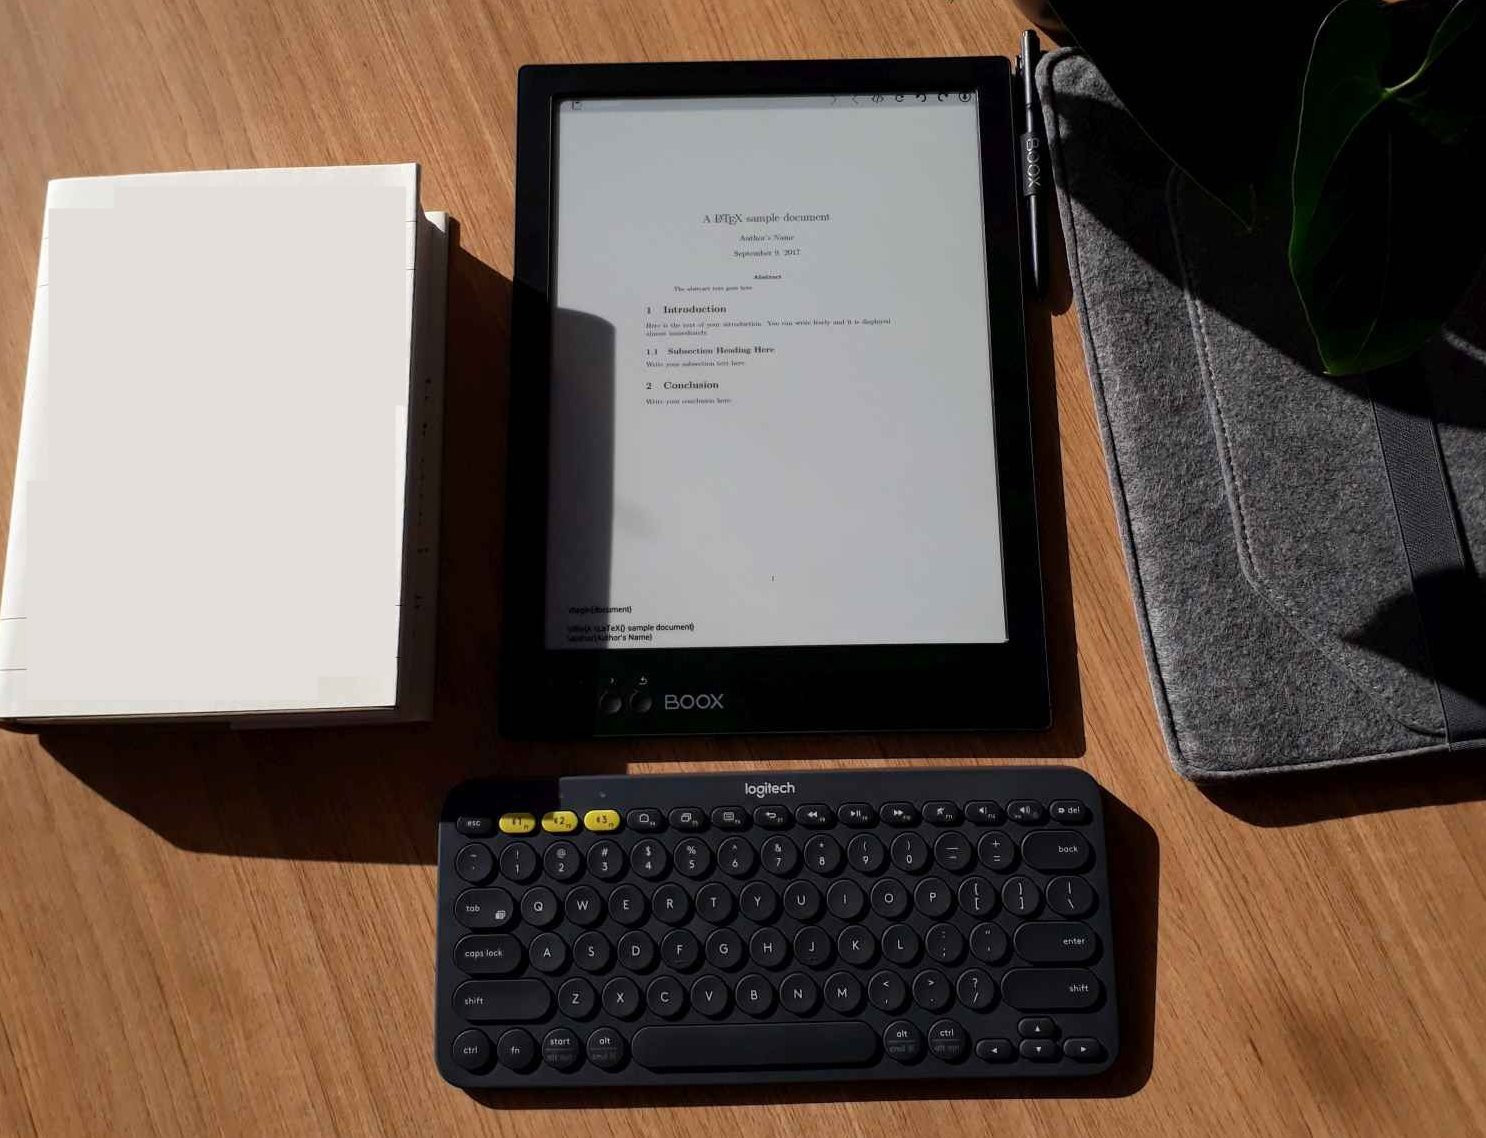
\includegraphics[width=0.45\textwidth]{figures/keyboard1}
\caption{General Hardware Setup}
\label{fig:setup}
\end{center}
\end{figure}
	

Fig.\ref{fig:setup} demonstrates the general hardware setup of SwiftPad, consisting an 13.3-inch e-paper device and an optional wireless bluetooth keyboard. We argue that keyboards are so far the most reliable input instrument for SwiftPad because of their popularity and users' familiarity. Nevertheless, we will discuss the possibility of integrating other input technologies such as speech recognition and handwriting input in Section~\ref{sect:discussion}. 


The e-paper device is now running a set of software components, whose architecture is demonstrated in Fig.~\ref{fig:editingexample}.
The topmost layer is the user interface (UI). Its WYSIWYG editor enables users to view and edit the PDF documents in their print forms. 
One key insight of this UI layer is that it is fully implemented in modern web-based technology (i.e., HTML5, CSS3, and Javascript), which 
can deliver high portability among different e-paper devices, tablets and PCs. Besides the portability, the HTML5-powered user interface, compared with conventional PDF viewers, features higher interactiveness and faster rendering on devices with low-end specifications \cite{peroni2017research,wang2013onlineperformance}. This is crucial because most off-the-shelf e-paper devices only possess limited computation ability (e.g., single-core 1GHz ARM CPU).
% Moreover, the HTML contents are intrinsically editable, which facilitates the implementation of the WYSIWYG editor.

% One core component of the UI layer is the HTML5-powered PDF viewer/editor, which renders a PDF document with a set of html documents. 

The component beneath the UI is the system utilities, which provides the UI with the runtime environment and typesetting functionality. 
For example, the Webkit engine is in charge of parsing and rendering the HTML5 pages from the UI and the \LaTeX\ engine handles document compilation requests.
It is worth noting that, the typesetting engine has been enhanced with a userspace checkpoint technology, which reduces the compilation time by skipping the unmodified pages and makes the WYSIWYG editor more responsive.

% Note that the SwiftLaTeX engine can be executed either in a remote cloud or local devices depending on the network availability. 

% namely, character-level positioning between PDF elements and \LaTeX\ source codes.

% Particularly, to support local execution, the engine is compiled into a binary format named WASM and can be directly executed by modern browsers.

The bottom layer is the Operating System (OS), which provides an embedded Linux environment (Busybox) implemented with size-optimization and limited resources in mind. It also contains an enhanced e-paper display driver, which significantly improves the viewing experience of e-paper applications that require constant screen update. 

% The optimization also enables a wide range of future e-paper applications that simultaneously require constant screen update and high display quality. (\textbf{error})
% Notably the OS now can receive certain display-related hints from user interface designers to deliver more responsive screen update and to combat ghost effects.
% Note that unlike most off-the-shelf e-paper devices powered by resource-consuming Android OSs, SwiftPad adopts a lightweight system architecture enlightened by WPE OS \cite{wpeos}, which provides a higher system responsiveness and a longer battery life using fewer CPU and memory resources. Furthermore, SwiftPad extends the OS to provide better support for e-paper screens. Notably the OS now can receive certain display-related hints from user interface designers to deliver more responsive screen update and to combat ghost effects.

\begin{figure}[h]
\begin{center}
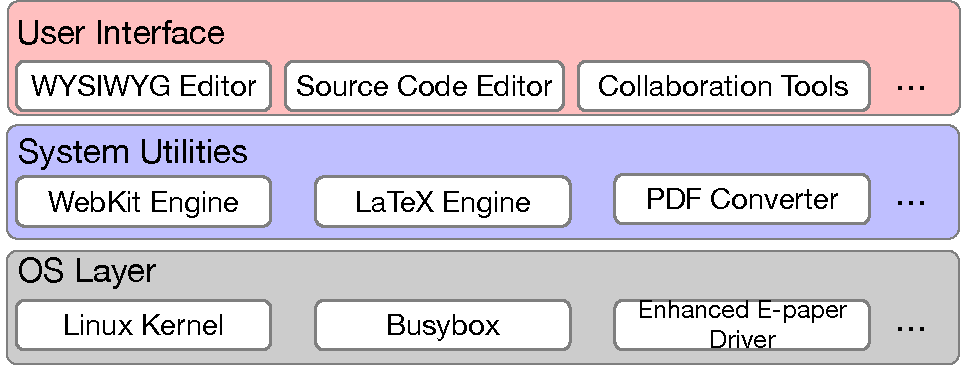
\includegraphics[width=0.45\textwidth]{figures/firefoxos}
\caption{System Architecture}
\label{fig:editingexample}
\end{center}
\end{figure}


Note that most off-the-shelf e-paper devices simply adopt Android OSs, which we argue is not an ideal solution.
Notably, Android has been designed to enable multimedia functionalities (e.g., gaming and video playback) in conventional mobile phones or tablets. Thus, Android comes with a great number of multimedia system services that are not utilized by e-paper devices. This leads to waste of system resources and unnecessary battery drain. In contrast, our system architecture is tailored for the e-paper devices with low specifications from the ground up. It is thus more resource-efficient and potentially provides a longer battery life.	

% provide , which help combat the notable drawbacks of e-ink screens including low refresh rate and ghost effects.

% recently has received a considerable amount of attention from smart device manufacturers \cite{}

% In the following sections, we will illustrate the challenging issues and corresponding solutions when implementing the above layers.
% In the following sections, we will illustrate the design and  for each layer, and discuss the challenging issues several techniques to cope with them.
% The layer can be further divided into two sub-layers including a bare Linux operating system and an enhanced webkit kernel. Specifically, the webkit kernel now can receive certain display related hints from web applications and to combat the notable drawbacks of e-ink screens including low refresh rate and gho{}st effects. 


\section{User Interface Design}\label{sect:htmleditor}

\begin{figure*}[t]
\begin{center}
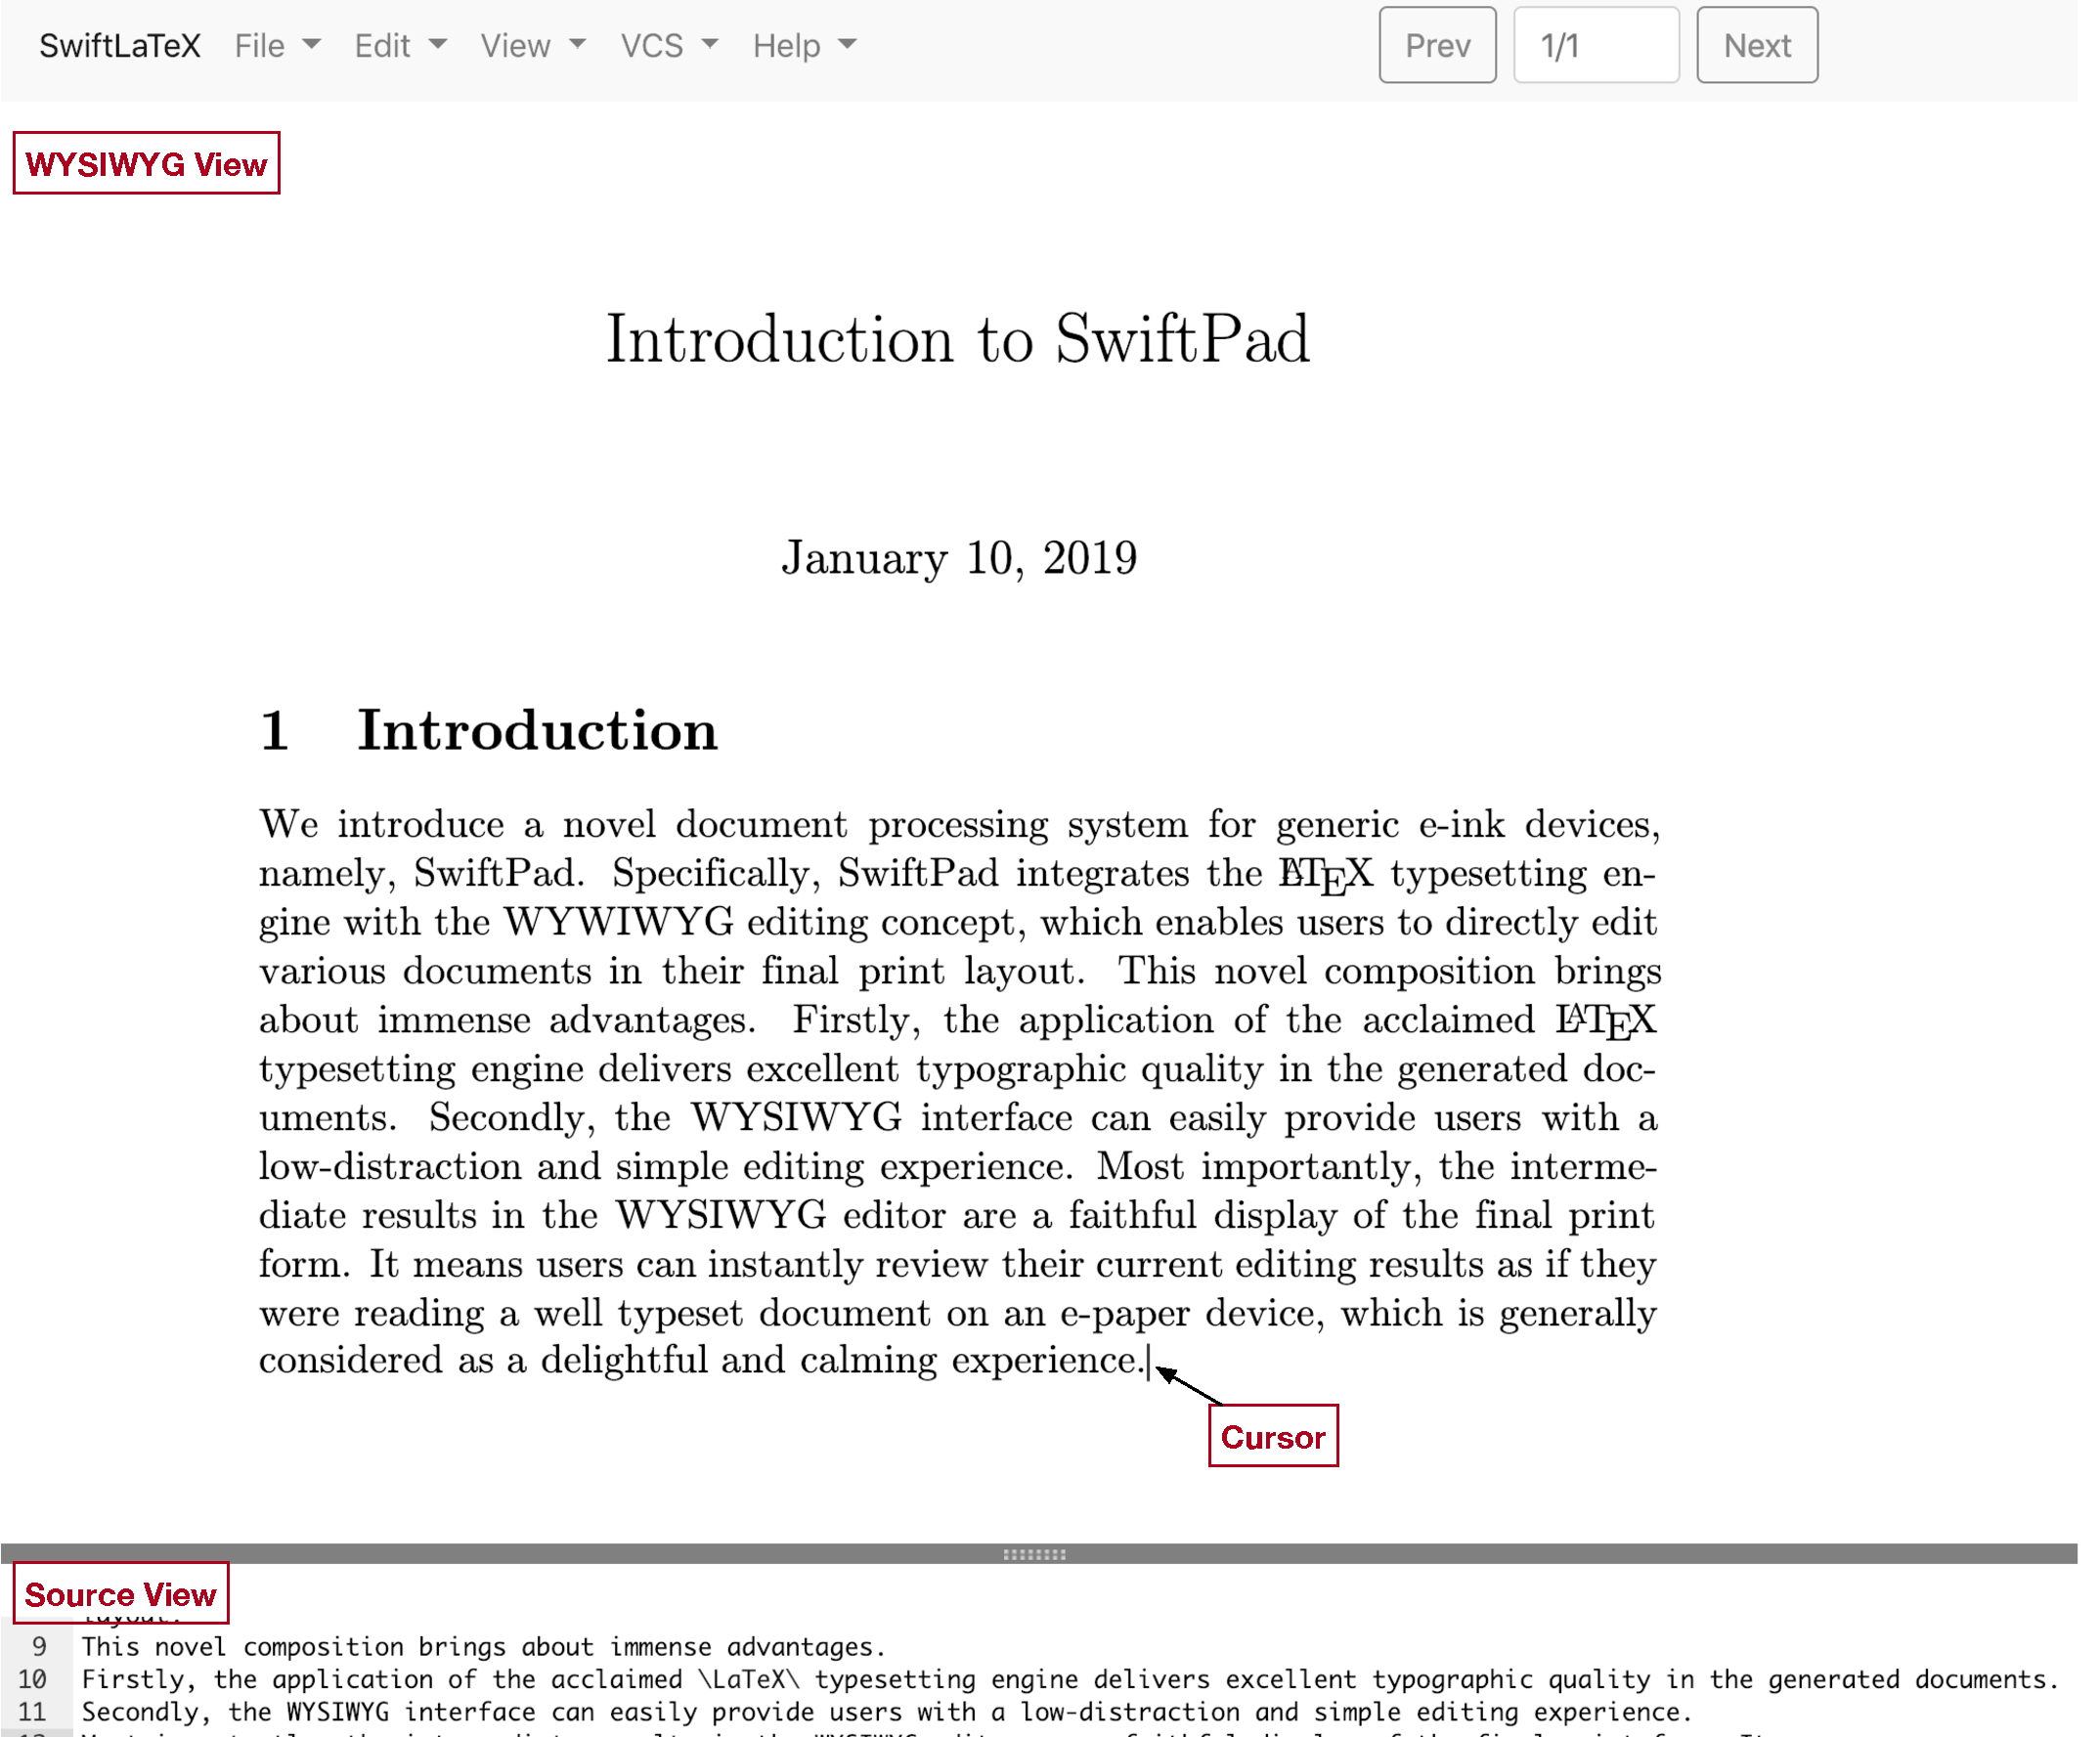
\includegraphics[width=0.8\textwidth]{figures/UIscreenshot}
\caption{User Interface of SwiftPad. }
\label{fig:uisc}
\end{center}
\end{figure*}
We design a simple-yet-powerful user interface for SwiftPad as shown in Fig.~\ref{fig:uisc}. Note that the screenshot is directly captured from a e-paper device's graphics memory in pursuit for better presentation purposes. It can be seen that SwiftPad offers two different editing views. 
The first one is the source view, which allows advanced users to directly manipulate \LaTeX\ source code in a classical ASCII editor.
This view needs to be preserved because only in source code can arbitrary \LaTeX\ scripting be done. 

 %(e.g., changing the document template or adjusting the page margin)  can be more conveniently altered in the source code. 
% Before we can elaborate the user interface design of our editor, we need to provide a precise definition for the notion of WYSIWYG editor for \LaTeX\. 
% In our paper,  a \LaTeX\ WYSIWYG editor should fulfill the following requirements: 

\subsection{A WYSIWYG Editor for \LaTeX}
Nevertheless, the main contribution lies in the WYSIWYG view.
This is an editable PDF viewer that allows the user to directly edit a document in its print form, but with effect on the source. More specifically, the viewer possesses the following features:
\begin{enumerate}
\item At editing quiescence (i.e., a moment when the editor has processed all previous edits of the user, and there are hence no pending edits that would further change the output), the editor shows the print layout of the PDF document, i.e., acts as a faithful print viewer. 
\item At editing quiescence, the user can position the cursor anywhere in the document with the mouse/touchscreen, arrow keys or a combination thereof.
\item The user can perform edits at the cursor position by simply typing the keys or backspace and get immediate feedback in the sense that the editor shows a \textit{preview version} of the print view. This is mainly achieved by mimicking the typesetting behavior used in the \LaTeX\ engine. For instance, when a character is being appended, it will automatically inherit the font settings from the previous characters to make itself visually agreeable.
\item To retain the modification, the user's editing operations will also be applied at the corresponding position of the \LaTeX\ source code. (This requires the editor to possess the ability to infer the source code position of each element in the PDF with character-wise accuracy. 
In our implementation, we achieve this with the help of a \LaTeX\ plugin introduced in the work \cite{elliott2018}. In short, the plugin enables position inference by patching the typesetting engine with a bookkeeping mechanism, where it constructs a position record for each character in the input source file and output them to the PDF file as metadata (also known as `Tagged PDF'). The position info in the PDF then can be retrieved by our specifically-designed editor, while being safely ignored by the conventional PDF viewers. )
\item If the user input pauses, the editor reaches editing quiescence automatically in a reasonable amount of time. It is achieved by replacing the current preview version with the latest compilation result, i.e., faithful output, from the \LaTeX\ engine.
\end{enumerate}
These features also constitute a precise definition for the notion of a WYSIWYG editor for \LaTeX\ used in our paper. We envision that such a WYSIWYG editor is satisfactory for e-paper devices where a sufficiently large proportion of scientific/technical documents could be edited.


\begin{figure}[t]
\begin{center}
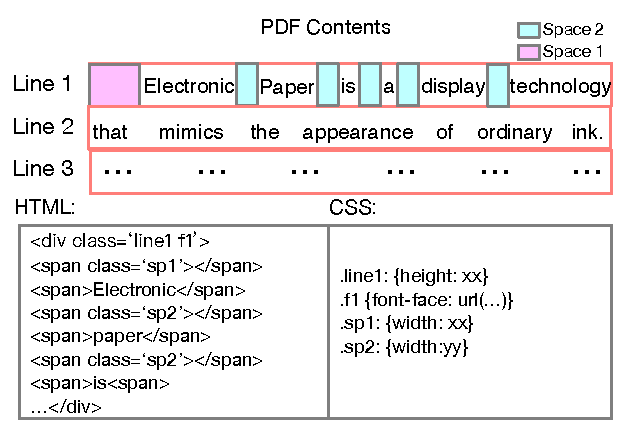
\includegraphics[width=0.45\textwidth]{figures/htmlconvert}
\caption{Workflow of the conversion algorithm}
\label{fig:convertexample}
\end{center}
\end{figure}
% built on top of the HTML5 and Javascript technologies. Briefly speaking, the viewer is able to render a PDF on the screen with a set of HTML5 elements.
% To start an edit, the user simply clicks on any visible text that should be modified. 
% A text cursor will appear indicating that the viewer is now ready for the user's input as shown in Fig~\ref{fig:editingexample} (a).
% Afterwards, all editing operations such as character appending or removal will instantly be  rendered on the viewer (i.e., \textit{preview version} of the PDF).
% %The viewer offers the user with an immediate impression of what the modified document will look like, in other words, a \textit{preview version} of the  PDF.
% Meanwhile, to retain the modification, the user's editing operations will also be applied at the corresponding position of the \LaTeX\ source code. After the re-compilation process, the user will automatically be presented with the new \textit{revised version} of PDF. 

% \subsection{Enable Direct Editing of PDF Documents}





\subsection{Faithful Conversion from PDFs to HTMLs}
To implement such a WYSIWYG editor, our system has to support not only faithful display, but also dynamic modification of PDF contents (i.e., instantly generating the preview version in response to the user's input). 
However, it is considered challenging because a PDF document is essentially a vector graphic, which is difficult to edit.
Though there exist a limited number of commercial closed-source products (e.g., FoxIt PhantomPDF viewer \cite{foxitreader}) which support simple `touch
up' operations such as adding or removing words, we argue that these solutions are not directly applicable for e-paper devices. First, they are originally designed for PCs and tend to pose unacceptable computational burden on resource-constrained e-paper devices. Moreover, these products are generally not portable among devices with different hardware specifications and software architectures.


To address these issues, we explore a novel approach to implement the WYSIWYG view by converting PDFs to HTML pages in a nearly faithful manner. Displaying HTML pages brings about a wide range of advantages. First, HTML pages are of high portability and can be displayed in various devices equipped with browsers. Meanwhile, rendering HTML pages in modern browsers is a relatively lightweight operation even for devices with low-end specifications. Most importantly, unlike vector-based PDFs, HTML pages are semantic-based; texts in HTML pages are typically surrounded by HTML semantic markup, which allows them to be dynamically modified with the help of Javascript. It facilitates the implementation of commonly-used word processing functionalities (e.g., text selection, insertion, deletion, copying and pasting) in the WYSIWYG view.

% by registering corresponding handlers for keyboard and mouse events.

To achieve a nearly faithful conversion, SwiftPad employs the following mechanisms to preserve the following kinds of elements in PDFs. 

\textbf{Images.} PDF supports graphical instructions such as drawing and image embedding. To preserve the graphic elements, we rasterize them into bitmap images, which then can be displayed using the CSS sprite technique \cite{souders2008high}.

\textbf{Font Embedding.} Fonts can be embedded in a PDF file, which ensures that readers always see the text in its original font. To preserve the fonts in a PDF, we extract all the fonts from the PDF and convert them into web open font types (WOFF) with the help of two third-party libraries MuPDF \cite{mupdf} and FontForge \cite{williams2003font}. The converted fonts then can be embedded in HTML pages using a CSS rule named `font-face' \cite{souders2008high}. 


\textbf{Text Locations.} Text elements are positioned with absolute coordinates in a PDF document. To preserve the locations in the HTML pages, one naive method is to convert the locations into CSS absolute position rules and assign them to HTML text elements. However, since each text segment is now associated with a unique CSS rule, the	page may be too bulky to store and transfer. Moreover, the absolute positions are not flexible; when a user inserts or deletes some texts, 
a large number  of CSS position rules must be changed accordingly in order to achieve text reflow functionality.	

Inspired by a more recent tool \cite{wang2013online}, we attempt a relative positioning method to position each text segment. A simple example in Fig.~\ref{fig:convertexample} demonstrates the intuition of our approach. Specifically, we first attempt to merge PDF text segments to text lines based on their geometric metrics. Afterwards, we measure the space width between words in each line and turn them into CSS rules. Finally, these rules can be used to construct HTML spacer elements (i.e., empty span elements in a certain width) to help position each text element from left to right in each line.
The advantage of this approach is that the number of generated CSS rules tends to be tiny since there are usually limited number of spacers with different widths in a PDF page. We can further reduce the number by merging some rules which have nearly identical width values at the cost of faithfulness in text locations. As a result, this approach can generate HTML pages with a much smaller size compared with the naive approach. 
Another important advantage is that this positioning method automatically enables text reflow functionality to a certain extent when texts are inserted or deleted.  
% It can be seen that the number of generated CSS rules is tiny since they are usually referenced by multiple HTML elements.




\section{Achieving High Responsiveness}\label{sect:checkpoint}





% \textbf{Talk about just one page}
% Conventional \LaTeX\ engines, due to their batch-style nature, typically feature a long turn around time of each compilation.
% which inevitably degrades the user experience as users may have to wait noticeable timespan to view the faithful output.
One essential requirement for WYSIWYG editors is high responsiveness; it allows users to instantly see what the end result will look like while a document is being  edited. In the context of SwiftPad, when a user types a key, our editor provides immediate response in the sense that it generates and shows a preview version of the document by mimicking the typesetting behavior used in the \LaTeX\ engine. 
Though the typesetting imitation approach is feasible for minor editing, it possesses certain limits when dealing with lengthy edits.
As a consequence, without any further precautions, the difference between the previewing version and the faithful output from the \LaTeX\ engine would gradually accumulate along with the user's input. To address this issue, our editor periodically replaces the current preview version with the latest compilation result from the \LaTeX\ engine.

However, this replacement operation potentially leads to unresponsiveness of our editor due to the long turn around time of each compilation.
 A complication process on conventional engines, depending on the complexity of the input source codes, can take several seconds to complete even on a computer with decent specifications (e.g., Intel i7 6900 with DDR4 memory and SSD storage). As a result, users may have to wait noticeable timespan in order to view the faithful output.

\subsection{Accelerating \LaTeX\ Compilation Using Checkpointing}
We find that the inefficiency of \LaTeX\ engines may be attributed to the following two reasons.
First, the \LaTeX\ engine, which was programmed decades ago, does not utilize the multi-threading feature of the modern machines. Thus, its execution speed is bounded by the clock rate of a single CPU core regardless of the number of cores.
Secondly, \LaTeX\ is a batching system, which implies that every time a compilation is initiated, the \LaTeX\ engine must process the input files from the very beginning. Such behavior is undesirable considering that, in most cases, users only append or modify characters located at the end of the input file, while leaving the preceding contents unchanged. Therefore, recompiling the unchanged contents leads to a considerable amount of repeated and unnecessary computation. 

To accelerate the complication process, one potential approach is to overhaul the source code of the \LaTeX\ engine to add multi-threading support. However, this requires extensive  reworking of the engines. More importantly, it may introduce unheeded bugs undermining the software stability.
Instead, we shift our attention on the second cause mentioned above and seek method to avoid the repeated computation between consecutive compilations.
The philosophy we apply here is called checkpointing, which consists of saving a snapshot of an application's state, so that it can restart from that point in the future. In the context of our enhanced \LaTeX\ engine, we create checkpoints periodically (e.g., after outputting a PDF page) and mark down the corresponding input file positions during the compilation process. When a new compilation job is submitted, based on the file position that users just edit on, the enhanced engine can determine the closest checkpoint and directly start from that point to skip the repeated computation.

Another optional trick to optimize responsiveness is that the engine does not have to process the whole input file in most cases. Instead, it may stop right after generating the page the user is currently viewing or editing. By combining this trick with the checkpoint technology, we can ensure the response time of the engine remains nearly constant regardless of the page number of documents. For instance, when the user is working on page 5, the engine can start from the checkpoint, which was generated when page 4 was being outputted, and only re-typeset the page 5. Though in some rare situations, contents from page 6 onwards may slightly affect the typesetting results of the page 5. We argue that the infrequent loss of faithfulness is negligible and would not seriously impact the overall user experience.

% To implement the checkpoint functionality, one naive approach would be to directly modify and extend the source code of \TeX\ engines. However, as we discussed in Section~\ref{wysiwyg}, such an approach is not recommended from a standpoint of software reliability engineering. To avoid the source code modification, we instead adopt a  runtime checkpoint approach. 

\subsection{Userspace Checkpoint Technology for \LaTeX}
Several runtime checkpoint implementations have been proposed. Early implementations are mainly kernel-based \cite{hargrove2006berkeley}. They utilize a specially-designed kernel module to save or restore process-related data structures in the kernel. However, the existing in-kernel implementations do not focus on upstream compatibility. As a result, it is very difficult to integrate them into recent mainline kernels and these implementations are therefore not further developed and abandoned.
To solve the issues of the in-kernel implementations, CRIU \cite{emelyanovcriu} proposes another approach; it implements as much functionality as possible in the user space and solely uses existing kernel interfaces. Despite the promising features of CRIU, it is a relatively heavyweight solution since it was originally designed for virtual machines or containers. It thus has to checkpoint a wide range of system-wide information not utilized by the \LaTeX\ engine (e.g., TCP sockets and process trees). This results in inefficiency of each checkpoint operation, which can take multiple seconds to finish.


These issues motivate us to propose a lightweight userspace checkpoint technology for the \LaTeX\ engine. Specifically, we utilize the dynamic hooking technique \cite{hooking} to patch the engine on the runtime with the checkpoint logic. Each checkpoint operation solely saves three types of information including \\	
1) CPU registers (e.g., Instruction Pointer) \\
2) memory segments including data, bss and heap \\
3) file position for each open file \\
and thus can be swiftly carried out (usually in less than 50 ms).

To fully recover the state of the \LaTeX\ engine, a special mechanism is required for memory segments. At first glance, restoring memory segments seems quite straightforward; we could simply write back the contents from the dump file to the original memory addresses. However, it is highly likely to fail due the stateful nature of the heap segment. Unlike data or bss segments whose sizes are pre-determined during the compilation, the size of the heap segment can vary constantly during the runtime. Specifically, when an executable allocates/releases a memory block via the standard C library calls `malloc'/`free', these functions internally invoke a system call `sbrk' to extend/shrink the heap segment. To efficiently manage the heap segment, the standard C library has to keep track of an important system state, namely, the current heap segment size. When the program is recovering from a checkpoint, in order for the C library to continue functioning properly, this system state has to be restored as well. However, the restoration functionality is generally not available in popular runtime C libraries (e.g., libc). 


% Therefore, before writing back the checkpointed heap data to the heap segment, we must ensure the current size of the heap segment is the same as the one in previous run.
% in. However, the restoration functionality is generally not available in popular runtime C libraries (e.g., libc). 

To address this issue, we patch the built-in heap allocator in the runtime C library such that rather than \textit{sbrk}, it now uses \textit{mmap} as the basic mechanism to obtain memory from the system. The advantage of using mmap is that it allows us to create a heap memory region that has been assigned a direct byte-for-byte correlation with a filesystem object. By duplicating the file, we will be able obtain to a snapshot of the heap memory region. To restore the region, we could simply map the snapshot file back to memory using \textit{mmap} again. This approach ensures that not only the heap segment contents, but also the heap segment size can be correctly restored across runs. 

% Note that no extra operation is required to recover the internal state of the heap segment since all the bookkeeping info is stored in the allocated heap region too. 

Special care is also given to the file objects, which are kernel objects and do not persist between runs. To address this issue, we will re-initialize every file object by reopening them and restore their file pointer positions by using the function \textit{fseek}.



To demonstrate the efficiency of our approach, we compare the compilation time of the conventional \LaTeX\ engine and our optimized engine in a same device with a single-core 1GHz ARM CPU and 512 MB RAM. Specifically, we first use a predefined set of \LaTeX\ code snippets to randomly generate a variety of \LaTeX\ sample documents, whose page numbers range from 1 to 100. Afterward,  
we insert texts at random places of each document and then start the compilation. Such a procedure will be repeated 100 times for each document and the average compilation time will be reported. 
 % In details, we utilize the `time' command to time the typesetting engine and the converter as they are user-space programs. On the other hand, to time the display operations of e-paper screens, we have to extend an interrupt handler of the kernel driver to capture the finish signal emitted by the e-paper screens.
The results are demonstrated in Fig.~\ref{fig:time}. It can be seen that the compilation time of the conventional \LaTeX\ engines increases proportionally with the page number of the \LaTeX\ documents. In the worst case, the 100-page document even consumes approximately 13 seconds.
We again conduct the measurements on our optimized engine. It can be seen that, regardless of the page number, the compilation time stays level (112 ms), which ensures high responsiveness to our editor. 

\begin{figure}[t]
\begin{center}
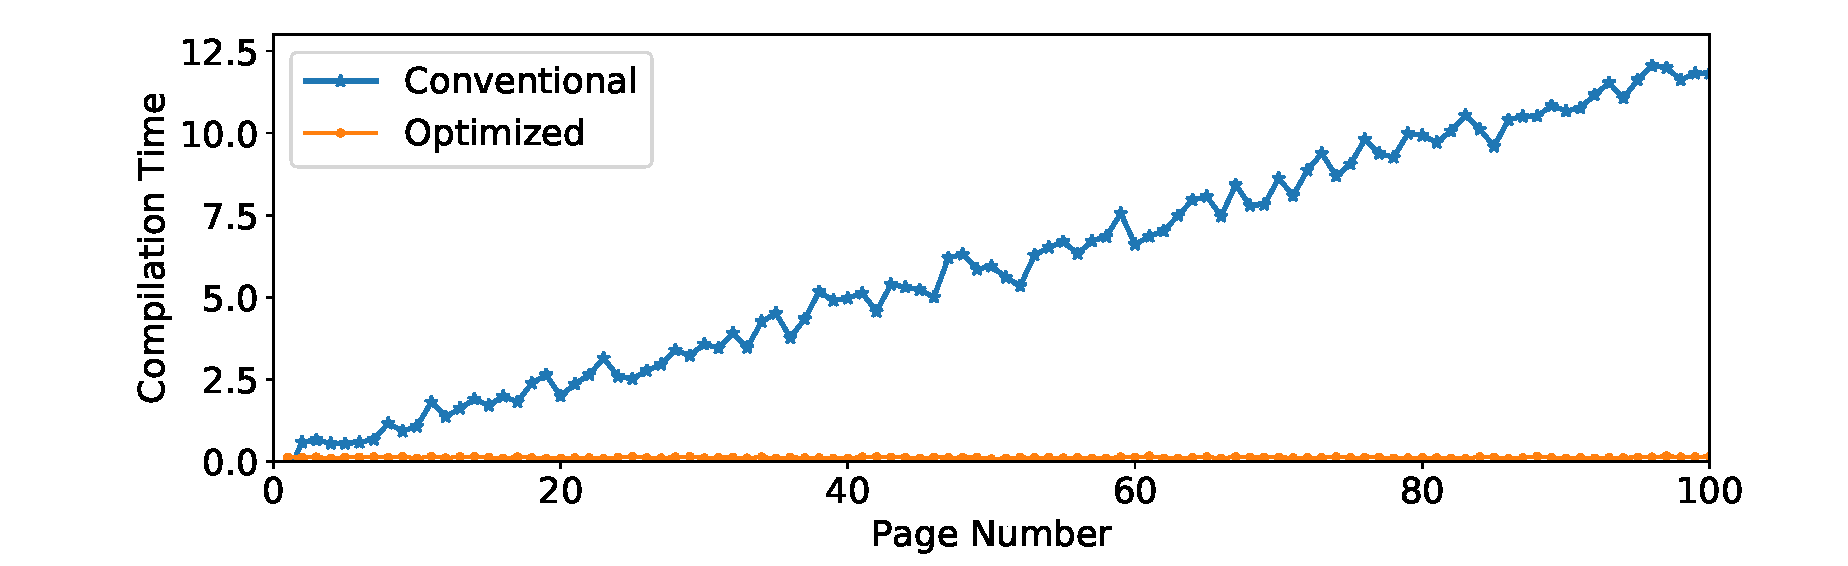
\includegraphics[width=0.45\textwidth]{figures/time}
\caption{Compilation time comparison between the conventional Engine and the enhanced engine.}
\label{fig:time}
\end{center}
\end{figure}

% It is mainly attributed to that our enhanced engine can skip a great amount of repeated computation by using checkpoint and solely generate one page output each time.

% Noticing that our editor only displays one page of documents each time, we could slightly

 % To efficiently manage the heap segment, the standard C library keeps track of two internal states including 1) occupied/free space in the heap segment and 2) the overall heap segment size.  When restoring the heap segment, these states have to be recovered correspondingly as well. However, the restoration functionality is missing in the most runtime C libraries (e.g., libc). 

% At first glance, restoring memory segments seems quite straightforward; we could simply write back the contents from the dump file to the original memory addresses. However, it is doomed to fail due to following two reasons. The first one stems from the system security mechanism named `address space layout randomization' (ASLR), which randomizes the location where applications are loaded into memory. Therefore, the memory addresses of each segment are different across different runs. To address this issue, we temporally disable the ASLR security mechanism for the TeX executable by setting its personality flags \cite{}. To ensure not to undermine system security, we apply a protection technology named `cgroup', which runs the executable with isolated system resources (e.g., filesystem and process space). Even if attackers manage exploit the vulnerability of the executable, they can only inflict limited harm on the system.

% The second issue derives from the stateful nature of the heap segment.  Unlike data or bss segments whose sizes are pre-determined during the compilation, the size of the heap segment can vary constantly during the runtime. Specifically, when an executable allocates/releases a memory block via the standard C library calls `malloc'/`free', these functions internally invoke a system call named `sbrk' to extend/shrink the heap segment. To efficiently manage the heap segment, the standard C library keeps track of two internal states including 1) occupied/free space in the heap segment and 2) the overall heap segment size.  When restoring the heap segment, these states have to be recovered correspondingly as well. However, the restoration functionality is missing in the most runtime C libraries (e.g., libc). 

% In our work, we modify the built-in heap allocator in the runtime C libraries such that rather than \textit{sbrk}, it now uses \textit{mmap} as the basic mechanism for obtaining memory from the system. By using \textit{mmap}, we are able to create a heap memory region that has been assigned a direct byte-for-byte correlation with a filesystem object. By simply duplicating the file, we will be able obtain a snapshot of the heap memory region. To restore the region, we could simply map the snapshot file back to memory using \textit{mmap} again. Note that no operation is required to recover the internal state of the heap segment since we store all the bookkeeping info in the allocated heap region.

% \textbf{Restoring Memory Segments} At first glance, restoring memory segments seems quite straightforward; we could simply write back the contents from the dump file to the original memory addresses. However, it is doomed to fail due to following two reasons. The first one stems from the system security mechanism named `address space layout randomization' (ASLR), which randomizes the location where applications are loaded into memory. Therefore, the memory addresses of each segment are different across different runs. To address this issue, we temporally disable the ASLR security mechanism for the TeX executable by setting its personality flags \cite{}. To ensure not to undermine system security, we apply a protection technology named `cgroup', which runs the executable with isolated system resources (e.g., filesystem and process space). Even if attackers manage exploit the vulnerability of the executable, they can only inflict limited harm on the system.

% The second issue derives from the stateful nature of the heap segment.  Unlike data or bss segments whose sizes are pre-determined during the compilation, the size of the heap segment can vary constantly during the runtime. Specifically, when an executable allocates/releases a memory block via the standard C library calls `malloc'/`free', these functions internally invoke a system call named `sbrk' to extend/shrink the heap segment. To efficiently manage the heap segment, the standard C library keeps track of two internal states including 1) occupied/free space in the heap segment and 2) the overall heap segment size.  When restoring the heap segment, these states have to be recovered correspondingly as well. However, the restoration functionality is missing in the most runtime C libraries (e.g., libc). 

% In our work, we modify the built-in heap allocator in the runtime C libraries such that rather than \textit{sbrk}, it now uses \textit{mmap} as the basic mechanism for obtaining memory from the system. By using \textit{mmap}, we are able to create a heap memory region that has been assigned a direct byte-for-byte correlation with a filesystem object. By simply duplicating the file, we will be able obtain a snapshot of the heap memory region. To restore the region, we could simply map the snapshot file back to memory using \textit{mmap} again. Note that no operation is required to recover the internal state of the heap segment since we store all the bookkeeping info in the allocated heap region.



% % It enables to such regions and to "pick up where it left off" when such regions are later dynamically mapped back in.,  
% % 1) By using mmap, it is easy to create heaps which are intended to be persistent and exist as a filesystem object after the creating process has gone away.
% % 2) Because multiple heaps can be managed, data used for a specific purpose can be allocated into its own heap, making it easier to allow applications to "dump" and "restore" initialized malloc-managed memory regions. For example, the "unexec" hack popularized by GNU Emacs could potentially go away.

% \textbf{Restoring File Descriptor ToDo}
% Restoring file descriptors is also tricky since they are kernel objects and do not persist among different run. 
% To address this issue, we utilize \textit{fopencookie}  to create a custom implementation for a standard I/O stream. This implementation can
% store the stream's data at a location of its own choosing; we provides a stream interface to data that is stored in a buffer in
% memory. 





% The causes are three-folded. The first one stems from the system security mechanism named `address space layout randomization' (ASLR), which randomizes the location where applications are loaded into memory. Therefore, the memory addresses of each segment are different across different runs. To address this issue, we temporally disable the ASLR security mechanism for the TeX executable by setting its personality flags \cite{}. Noticing that disabling ASLR might leave the executable vulnerable to attacks, we apply a protection technology named `cgroup', which run the executable with isolated system resources (e.g., filesystem and process space). Thus, even attackers manage exploit the vulnerability of the executable (which is unlikely), they can only inflict limited harm on the system.

% The second issue derives from the stateful nature of the heap segment.  Unlike data segments whose sizes are pre-determined during the compilation, the size of the heap segment can vary constantly during the runtime. Specifically, when an executable allocates/releases a memory block via the standard C library calls `malloc'/`free', these functions internally invoke a system call named `sbrk' to extend/shrink the heap segment. To efficiently manage the heap segment, the standard C library keeps track of states including occupied/free space in the heap segment and the current heap segment size.  When restoring the heap segment, these states have to be recovered correspondingly as well. However, the restoration functionality is still missing in the state-off-the-art implementations of the runtime C libraries (e.g., libc).

% whose main principles are also applicable in various applications apart from the \TeX\ engines.  



% \subsection{Kernel-based vs Userspace-based Checkpointing}

% We first conduct a detailed survey of the commonly-used checkpointing implementations. They can be mainly divided into two categories, namely, kernel-based and userspace-based.

% The kernel-based techniques utilize a specially-designed kernel module to save or restore process-related data structures in kernel (e.g., process control block and file descriptor table). The approach, however, possesses two significant drawbacks including questionable stability and poor compatibility. Regarding the stability, it is not difficult to see that a kernel module, if under-optimized, is likely to degrade the operating system's performance. Moreover, its unheeded bugs  could have severe consequences on the system (e.g., data loss or elevated privilege vulnerability). As for the compatibility, due to fast-paced kernel upgrade, the internal data structures in kernel may vary drastically across different kernel versions. Thus, kernel modules have to be specifically tailored for each version, which involves extensive human labor and can be demanding. For instance, the most well-known kernel-based implementation, the Berkeley Lab Checkpoint/Restart system \cite{hargrove2006berkeley}, has not been updated for almost half a decade and can only work on an obsolete kernel (Linux 2.6.37).

% In contrast, the userspace-based implementations seem a more plausible solution.
% In terms of stability, a userspace program, even poorly-implemented, barely inflicts harm on the operating system's stability. 
% As for the compatibility, regardless of the constant upgrade of kernels, the application programming interfaces (APIs) exposed to user space generally remain unchanged. It then allows unmodified userspace programs to run smoothly across different kernel versions. Owning to these promising features, our system adopts the userspace-based implementations.

% One the-state-off-the-art implementation is named `Checkpoint/Restore In Userspace' (CRIU) \cite{emelyanovcriu}. However, we argue that it is not an ideal option for our system owning to the following reasons. First, CRIU is a relatively heavyweight solution since it was originally designed for virtual machines/containers. It consumes a considerable length of time (up to seconds for a single process) checkpointing/restoring abundant information (e.g., sockets, virtual memory area, and process tree). Most of the information, however, is not utilized by the \TeX engine. More importantly, in order for CRIU to work properly, a considerable number of advanced kernel features must be presented. However, this requirement may not always be met for certain machines. 

% Based on the above argument, we propose a novel checkpointing technology which is lightweight and solely relying on common kernel features including memory allocation and file operation. Note that the principles of our approach can be generally applied on a majority of single-threaded applications.



% % \subsection{Persisting Heap Space}
% One crucial step is to save and restore the contents of virtual memory belonging to the application.
% We demonstrate the memory content layout in Fig. It can be seen that the memory contents can be roughly divided into three major components including data/bss segments (initialized/zero-value global or static variables), heap segments (dynamic allocation) and segments used by system libraries. The figure also illustrates some pointer variables, whose values are the memory address of another value located in another segments. One special pointer  is called file pointer, which contains information about the file being opened such as its name and current position of the file.

% Saving these segments is relatively straightforward, for instance, using the system call named `write' to store the memory contents to a file. In contrast, restoring the memory contents from the dump file can be challenging. Simply writing back the contents from the file to the original memory addresses is almost doomed to failure. 

% The causes are three-folded. The first one stems from the system security mechanism named `address space layout randomization' (ASLR), which randomizes the location where applications are loaded into memory. Therefore, the memory addresses of each segment are different across different runs. To address this issue, we temporally disable the ASLR security mechanism for the TeX executable by setting its personality flags \cite{}. Noticing that disabling ASLR might leave the executable vulnerable to attacks, we apply a protection technology named `cgroup', which run the executable with isolated system resources (e.g., filesystem and process space). Thus, even attackers manage exploit the vulnerability of the executable (which is unlikely), they can only inflict limited harm on the system.

% The second issue derives from the stateful nature of the heap segment.  Unlike data segments whose sizes are pre-determined during the compilation, the size of the heap segment can vary constantly during the runtime. Specifically, when an executable allocates/releases a memory block via the standard C library calls `malloc'/`free', these functions internally invoke a system call named `sbrk' to extend/shrink the heap segment. To efficiently manage the heap segment, the standard C library keeps track of states including occupied/free space in the heap segment and the current heap segment size.  When restoring the heap segment, these states have to be recovered correspondingly as well. However, the restoration functionality is still missing in the state-off-the-art implementations of the runtime C libraries (e.g., libc).

% In our system, a novel heap state save/restoration mechanism is proposed. During the implementation, we realize that the most challenging step is the restoration of the heap segment size across different runs. Naively, we can control the heap size via the system call `sbrk' as the standard system library does. However, it is not an ideal solution due the unpredictable behavior of `sbrk'. First of all, the system call, under certain circumstances, may create a heap segment starting at a random memory address. More importantly, the `sbrk' can only extend/shrink at a limited size (e.g., 4MB in Linux) during each invocation. It renders the restoration of large heap segment inconvenient. (Todo:) Instead, we utilize an alternative system call named `mmap', which conveniently allows us to obtain a memory area at a fixed memory address with an arbitrary size. More importantly, the memory area can also be mapped to a filesystem object.

% The last issue stems from the system segment.
% By using mmap, it is easy to create heaps which are intended to be persistent and exist as a filesystem object after the creating process has gone away.
% The difficulty of restoration lies in the uncertain behavior of the system call `sbrk'. Specifically, the system call may extend the heap segment with an unpredictable size depending on a set of factors. 

% It poses an obstacle to reinstall the memory when restoing an application, i.e., how to persist the heap state of each run, such that pointers in data/bss segments can be still vaild.

% Nevertheless, the addresses the sbrk returns can vary drastically depending on many factors.

% One essential challenge is the randomization of heap memory allocation. Unlike the data segments that are usually located at the same memory address among different runs, the heap segments contains much more uncertainty.


% The application state of a single-threaded applications is mainly decided by the following three components: 1) the program counter, 2) virtual memory contents, and 3) opened file handles. 

% To implement the checkpoint/restore functionality, one cruical step is to dumping/reinstall the memory contents of the data/bss segments and the heap. Dumping is relatively easy (e.g., using fwrite to save the contents to a file) while reinstalling is a bit tricky due to the heap address difference between each run of an application.

% More specifically, traditional heap allocation relies on the system-built in functions (i.e,m malloc/calloc/realloc/free). These functions internally utilizes sbrk system call to obtain memory from the kernel. Nevertheless, the addresses the sbrk returns can vary drastically depending on many factors (e.g., whether the kernel enables address randomization and how much memory is requested, etc). It poses an obstacle to reinstall the memory when restoing an application, i.e., how to persist the heap state of each run, such that pointers in data/bss segments can be still vaild.


% \subsection{Restoring File Descriptor}


\section{Optimizing the E-paper Display Driver}\label{sect:os}
Existing e-paper devices are mainly designed for displaying static contents. As a result, they are not well optimized for applications like the WYSIWYG editor, which requires constant screen update. In this section, we will elaborate our enhancement to the e-paper display driver to address this issue. 



% This architecture is optimized for embedded and low-consumption computer devices.
% Compared with the Android OS, this integrated design significantly reduces platform overhead without sacrificing performance or a rich user smart phone experience. 
% The OS can be run in smart devices with low-specifications (128MB RAM and a single-core CPU) and provide a long-lasting battery life.



% The uppermost layer is the application, implemented in modern web programming languages (e.g., HTML5 and Javascript).
% The browser layer is the web engine that provides an HTML5 parsing and rendering engine as well as programmatic access to hardware functionality.
% The kernel layer then provides a set of drivers for the browser layer to control the underlying hardware (e.g., touchscreen and WiFi).
% Compared with the Android OS, this integrated design reduces platform overhead without sacrificing performance or a rich user smart phone experience. 
% The OS can be run in smart devices with low-specifications (128MB RAM and a single-core CPU) and provide a long-lasting battery life.





% \subsection{Enhancing graphics driver for e-paper screens}


% Graphics stacks in most existing OSs are designed for conventional LCD screens which can refresh the whole screen contents in a high speed of 60 Hz upwards. However, state-of-the-art e-paper devices can only achieve a refresh rate up to 7 Hz. The low refresh rate demands certain optimization on the graphics stack.

% \textbf{major issue}


\subsection{How E-paper Screens Work?}
% In our work, we further customize the WPE OS to provide more comprehensive support for e-paper screens. 
Before we can demonstrate the intuition of our enhancement, we first explain the internal display mechanism of e-paper screens.
An e-paper screen is controlled by a specifically-designed circuit, the Electrophoretic Display Controller (EPDC). It is responsible for driving corresponding electrical signals to the e-paper panel to update the screen contents upon receiving display update commands from the CPU. 
Most update commands can be described as a tuple ($x$, $y$, $w$, $h$, $data$, $mode$). Specifically, the first five parameters denote the coordinate, size and content of the rectangle region pending to be updated. The $mode$ parameter denotes the update mode, whose possible options include 2, 4, 8, or 16 graylevels. 
The 16-graylevel update mode delivers the best display quality (i.e., highest contrast and little ghost effect) but consumes the longest timespan to finish (approximately 1 second).
The 2-graylevel update modes enables fast animation of the screen contents (approximately 150 ms) but may generate poor contrast texts and significant ghost effects.


To communicate with the EPDC, the OS requires a kernel driver. 
% However, most existing driver implementations possess an essential drawback on the update mode selection.
One important task of the driver is to composite a update request tuple.
The system can obtain the first five parameters (i.e., $x$, $y$, $w$, $h$, $data$) directly from the upper layer of the OS.
For the update mode, this info is typically not available since most OSs are designed for LCD screens which do not require the update mode information.
% the update mode for each request has to be inferred before the driver can submit it to the EPDC.
Therefore, the drivers have to provide a mechanism to infer the update mode.
However, most existing driver implementations possess an somewhat rudimentary update mode selection mechanism.
One of the most widely-used mechanisms is to provide a kernel interface to allow an application to manually specify the global update mode.
For instance, an application featuring constantly varied contents can enforce the 2-graylevel update mode; on the other hand, a reading application requiring high display quality can enforce 16-graylevel update mode.
However, this mechanism is relatively coarse-grained and may not be suitable for applications that simultaneously require fast response time and high display quality, so does our WYSIWYG editor.





 
% The other one is more sophisticated. through its histogram analysis feature.

% Note that the update modes are typically not available from the applications in the upper layer. Most drivers deploy a simple strategy to infer the update mode;  through its histogram analysis feature.
% First, most implementations place the incoming update requests in a queue and process them in the order they are received. 
% To speed up the update process, the driver attempts to detect those update requests whose update regions do not overlap.
% Note that most EPDCs support the simultaneous update operation; multiple update requests can be handled on the same moments if their update regions do not overlap.
\subsection{Heuristic Multi-queue Scheduling Algorithm for E-paper Display}

\begin{figure}[t]
\begin{center}
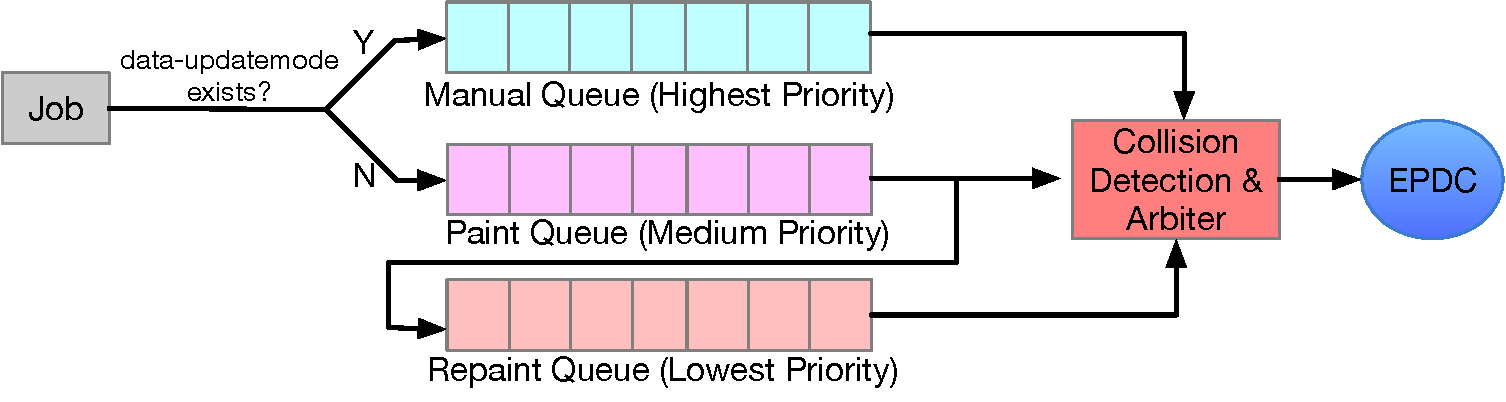
\includegraphics[width=0.45\textwidth]{figures/heruist}
\caption{Multi-Queue scheduling algorithm}
\label{fig:Heruist}
\end{center}
\end{figure}
In our work, we optimize the existing e-paper display driver to automatically strike a balance between the display quality and response time with a heuristic multi-queue scheduling algorithm.

As shown in Fig~\ref{fig:Heruist}, our algorithm maintains three separate update queues including a manual queue, a paint queue and a repaint queue. The manual queue is a simple queue which only stores the incoming jobs that have update modes specified by the developer.
Specifically, we enhance the Webkit browser engine with an interface, which enables the HTML applications to choose a desired update mode for each HTML element by using a HTML data attribute named \textit{data-updatemode}. For instance, when the browser is rendering the HTML text element \textit{\textless span data-updatemode=4\textgreater Open\textless span\textgreater}, the screen update request will be sent to the manual queue and later painted using the 4 graylevel mode.


% Such an interface may be useful for static UI elements (e.g., menus and text labels).

% When the value is set to be 16 or 2, the HTML element will be directly painted using the 16 graylevel mode or 2 graylevel mode respectively.

Nevertheless, most of the time developers do not manually specify the update mode. In this case, the paint and the repaint queue will be used. Specifically, 
the paint queue stores all the incoming update requests without update mode info from the application, which will then be sequentially drawn on the screen using 2-graylevel mode. Intuitively, this ensures the e-paper screen  display the latest contents as soon as possible (i.e., to deliver a responsive user experience).
After leaving the paint queue, the update job will enter the repaint queue and be later repainted again using 16-graylevel mode to improve the display quality (i.e., alleviate ghost effects and show high-contrast texts). In other words, if no new update jobs are submitted to the driver, the high display quality of the screen contents will eventually be achieved. 

This algorithm also takes advantage of the simultaneous update feature of the EPDC, which allows multiple update requests to be processed at the same moment when their update regions do not overlap with each other. In other words, the painting jobs and repainting jobs may be carried out simultaneously if their update regions do not collide. This condition frequently holds true for our editor application. A typically example has been depicted in Fig.~\ref{fig:drawing}; at stage one, the user types a word `hello', which is drawn in 2 graylevel mode. At stage two, the user types another word `world', this word is still drawn in 2 graylevel mode while the previous word `hello' can be repainted using 16 graylevel mode at the same time since the update regions of the two words do not collide. At the last stage, the user stops typing, so the word `world' is repainted and all the words are now in 16 graylevel mode.

Note that the max number of simultaneous update regions is decided by available hardware resources of the EPDC and may be quite limited. When the application is overloading the EPDC by submitting too many update requests at the same time, we prioritize the three queues to optimize the average screen response time (manual \textgreater paint \textgreater repaint).
For a update request in a queue to be executed, two conditions must be met; 1) the EPDC has available resources, 2) all the update requests in those higher priority queues should have either finished the execution or been scheduled (i.e., being drawn).
% To optimize the average screen response time, especially when the application is submitting too many update requests and overloading the EPDC, we decide to prioritize the three queues. 

% For a update request in a queue to be executed, all the queues of priority higher than it should be empty, meaning the update requests in those high priority queues should have finish its execution. 

% In some situations where the application submits too many update jobs and overloads the EPDC, we have to prioritize different queues. 

\begin{figure}[t]
\begin{center}
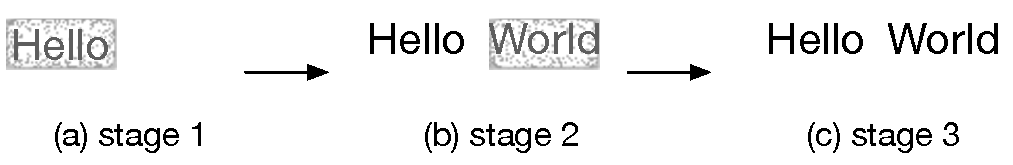
\includegraphics[width=0.45\textwidth]{figures/helloworld}
\caption{A demonstrating example of the scheduling algorithm}
\label{fig:drawing}
\end{center}
\end{figure}






% Meanwhile, to address the ghost effect issue, the update regions will be later repainted using 16-graylevel mode. 
% by taking advantages of the simultaneous update feature. 
% We place the incoming update requests in a queue and process them in the order they are received. 
% The repair stage can be carried out with the painting stage simultaneously.
% To speed up the update process, the driver attempts to detect those update requests whose update regions do not overlap.

% However, the automatic mechanism is not widely optimized. We provide a fine-grained mechanism to allow applications to select update modes for each UI component.

% responsibility for managing update order. Updates are processed in the order they are received by the EPDC.
%  also manually choose the appropriate waveform update mode.
%  contains only 2, 4, 8 or 16 gray levels.





%  Such an 

% B2G OS is a community-developed successor to Firefox OS, (developed by Mozilla Foundation). It follows the Firefox OS vision of providing a complete, community-based alternative operating system, that runs software as web applications. The software ('applications') therefore use open web standards and programming languages such as JavaScript and HTML5, a robust privilege model, and open web APIs that can communicate directly with the device's hardware.


\section{Evaluation}\label{sect:eve}
In this section, we demonstrate the settings and outcomes of our evaluation on usability of SwiftPad. 

\subsection{Experiment Devices}
In our experiments, we deploy SwiftPad on two popular off-the-shelf 13.3-inch devices BOOX MAX \cite{onyxboox} and reMarkable \cite{reMarkable}. 
The devices are built atop an NXP i.MX 6 Solo SoC \cite{nxpsoc}, which is equipped with a single-core 1Ghz CPU, 512MB DDR3 RAM and an EPDC. Since the SoC's bootloader and Linux kernel source codes are both publicly available on the Internet, we can easily modify the e-paper devices to meet our requirements (e.g., installing the enhanced e-paper driver). 
Note that since SwiftPad features an implementation with high portability, it takes little effort to port SwiftPad to other devices with different hardware architectures or screen sizes. 
% For development and debug purposes, we also build our own in-house hardware prototype which consists of an ES133UT2 13.3 e-ink screen, an IT8942 EPDC and an Intel NUC Mini PC running a desktop Linux distribution.

% Meanwhile, we build our own in-house hardware prototype which consists of an ES133UT2 13.3 e-ink screen, an IT8942 e-paper screen controller and an Intel NUC Mini PC. The PC is in charge of running the SwiftPad system and sending the drawing instructions to the e-paper screen controller. One essential advantage of the prototype is that the PC provides a set of development tools such that the developers can directly implement and debug each iteration of SwiftPad on the PC.

% \subsection{Performance Evaluation}
% One essential performance metric of SwiftPad is the response time, in other words, the time span between the moment a user initiates a keystroke and the moment the corresponding faith result appears on the screen. Specifically, the response time mainly consists of three major components including the compilation time of the typesetting engine, the render time of the output document, and the display time of the e-paper screen.

 
% In details, we utilize the `time' utility to time the \TeX\ engine and the converter as they are user-space programs. On the other hand, to time the display operations of e-paper screens, we have to extend an interrupt handler of the kernel driver to capture the finish signal emitted by the e-paper screens.

% As shown in Figure~, the compilation time of the conventional \LaTeX\ engines increases proportionally with the page number of the \LaTeX\ documents. In the worst case, the 200-page document even consumes approximately 10 seconds. It is expected and we have investigate the reasons of the lengthy compilation time in Section~.
% Clearly, the conventional \LaTeX\ engines are not suitable for the implementation of the WYSIWYG editor since users may have to wait noticeable timespan to view the faithful output. We again measure our \TeX\ engine with the incremental compilation feature enabled. It can be seen that, regardless of the page number, the compilation time stays level (approximately 50ms). 
% The short compilation time is mainly attributed to the fact that TeX engine can determine the closest checkpoint and directly start from that point to skip the repeated computation. 

% The render time of the output document consists of two major parts, the conversion from PDF to HTML as well as the HTML parsing and painting. Our results indicate that the 95\% confidence interval of the conversion time is [16.7 ms, 20.1ms]. The 95\% confidence interval for parsing and painting time is [16.3 ms, 22.1 ms].

% We also measure timespan for each display operation. As described in the Section~, the timespan is mainly affected by the update mode selected. Our measurements show that averagely, a 2-graylevel drawing operation consumes approximately 167 ms, while the 16-graylevel takes 1172 ms. Since the e-paper scheduling algorithm will try to paint the content in 2-graylevel mode, we can conclude that the minimum response time for SwiftPad is approximately 257 ms.



\subsection{Usability Evaluation}

The evaluation has been carried out as a Discount Usability Test, which involves a small number of participants with a focus on qualitative studies on prototype design \cite{nielsen1989usability}. Existing studies \cite{nielsen2015you}\cite{nielsen2009discount} have suggested that a discount usability test with only 5 participants can offer reliable evaluation results and may identify up to 85\% of the usability problems. In our work, we invited 6 participants from academia to evaluate our system and gathered many important insights and feedbacks.
In the near future, we are planing to carry out a comprehensive usability study, which involves more participants from different domains.

Before undertaking the test, each subject was instructed to fill in a short questionnaire, which contains the following categories of questions on a five-point scale (strongly disagree, disagree, neutral, agree, strongly agree):
\begin{itemize}
\item Frequency and enjoyment of writing.
\item Familiarity of e-paper devices (i.e., how often do they read in e-paper).
\item Experience in various typesetting programs.
\end{itemize}

After that, each participant was instructed to perform the following tasks in an unsupervised manner; the subjects had to finish each task by themselves without any prior knowledge of SwiftPad.
\begin{enumerate}
	\item The participants were required to compose an essay with at least 500 words, describing their current research focus. 
	\item Each participant was provided with an one-page English article on a topic of general interest. In each line of the article, there existed an obvious typo and the participants were supposed to correct it.
	% \item We provided each subject with a set of simple mathematical equations with incorrect calculation (e.g., $1 - \frac{1}{4} = \frac{2}{4}$). The participants were required to correct the final results of the equations.
\end{enumerate}

After completing these tasks, we required the participants to complete a System Usability Scale (SUS) questionnaire, which is a commonly-used reliable tool for perceived usability evaluation even with a small sample size.
We also encouraged participants to report their experience of using SwiftPad.

\textbf{SUS Score.}
The mean SUS score of SwiftPad is 71 (in a range spanning from 0 to 100). It exceeds the threshold score of 68 which  indicates a decent level of usability. 
In addition, we also compute the mean values for the usability sub-scale and learnability sub-scale, which are 70 and 75 respectively. 

Meanwhile, by considering participants' answers given in the background questionnaire, we obtain three more background sub-scores.
They are compared with the SUS score and sub-scale scores to obtain the Pearson correlation coefficients. 
We notice a weak positive correlation between the user's familiarity of e-paper and the learnability sub-score, which implies that users who get used to reading in e-paper devices may find it easier to master our system.
However, due to the small sample size, each correlation measure appears to be not statistically significant. To reach a more solid conclusion, a more comprehensive dataset is required.
% All the 6 participants actively responded to our invitation and we received 6 responses about the current prototype of SwiftLaTeX.

\begin{table}[t]

\centering

\caption{Axial coding of the participants' comments}
\label{tab:comments}

\begin{tabular}{|l|l|l|}
\hline
Categories                                                      & Positive & Negative \\ \hline
\begin{tabular}[c]{@{}l@{}}Paper-like viewing \\ experience\end{tabular}       & 6        & 0        \\ \hline
\begin{tabular}[c]{@{}l@{}}Aesthetics \end{tabular} & 5        & 0        \\ \hline
Simplicity                                                        & 4        & 0        \\ \hline
Low distraction                                                       & 2        & 0        \\ \hline
Latency                                                 & 1        & 3        \\ \hline
Keyboard input                                                & 0        & 1        \\ \hline
Structural change                                                & 0        & 1        \\ \hline
Math editing                                                & 1        & 1        \\ \hline
\end{tabular}

\end{table}

\textbf{User Feedback.}
All the participants' comments are summarized in Table~\ref{tab:comments} using Axial coding. 
On one hand, most participants praised the natural combination of excellent viewing experience of e-paper and print aesthetics of \LaTeX\ documents. 
Meanwhile, this system still maintains simplicity; with the WYSIWYG editor that possesses simple editing primitives and high familiarity with existing word processors, participants can efficiently concentrate on the actual document composition or editing without mastering the complex \LaTeX\ scripts. 
Two participants further commented that conventional PCs are usually equipped with noisy cooling fans and glowing screens leading to eye strain. In contrast, e-paper devices are quiet and their paper-like non-glowing screens provide a calming and almost distraction-free atmosphere for document writers.  




% 1) Excellent viewing experience, 2) Print aesthetics of \LaTeX\ documents, and 3) Calming and relaxing atmosphere.

% 1) innovative WYSIWYG editing for basic text and mathematical formulas, 2) the web-based interfaces, and 3) high efficiency for various kinds of editing tasks such as proofreading. 
% A participant also provides valuable insight into the benefit of fine-grained synchronization.
% Specifically, existing \LaTeX\ editors behave poorly in proofreading tasks mainly because of the coarse-grained synchronization functionality. 
% A word in PDF is commonly mapped to a lengthy line in the source code.
%  To modify the word, users are required to skim through the line to get the exact position of the word, which is fairly time-consuming. SwiftLaTeX successfully overcomes this issue by achieving character-level synchronization accuracy.
% Another participant who has little experience in \LaTeX\ applauded the smooth learning curve of SwiftLaTeX, which possesses high familiarity with the existing word processors but produces much more high-quality typesetting output.
% In addition, SwiftLaTeX allows users to focus on document composition without concerning about the complex script language and the time-consuming compilation and debugging process.

On the other hand, Table~\ref{tab:comments} also reveals some widely perceived issues. 
One important issue highlighted was the screen latency. 
Despite our effort to optimize the graphics stack, most participants, who get used to conventional LCD screens, can still perceive the display latency due to the hardware limit of e-paper screens.
Nevertheless, the participants were happy to accept the minor imperfection, which has limited impact on the usability of SwiftPad. One participant even provided an interesting argument that conventional typewriters tend to have much higher latency, however, impeding no functionality. 
% SwiftPad also has comparative advantages over typewriters in terms of flexible cursor positions.
Meanwhile, one participant encouraged us to explore other input technologies other than keyboard. He suggested that handwritten input would also be a natural input method for e-paper devices.
Another issue was the rudimentary functionality to apply structural changes (e.g., adding a new section or list structure). 
Currently, these structural changes could be applied via clicking the corresponding options in the context menu (i.e., pop-up menu).
However, one subject suggested us to mimic the autoformat features (e.g., automatic bullets or numbering) from Microsoft Word.
A related issue is about mathematical formulas editing. One subject noticed and praised the functionality of in-place mathematical formulas editing where users are allowed to change the text in an existing formula just like normal text. This functionality is quite useful in many scenarios, for instance, correcting the simple mathematical equations like $1 - \frac{1}{4} = \frac{2}{4}$. However, the subject also wished us to propose a method to insert or edit more complicated formulas without manipulating the \LaTeX\ source codes. 

% Alternatively, SwiftLaTeX could support Markdown language such that a simple snippet could be used to generate structural changes.
% Meanwhile, the majorities of subjects also complained about the invalidity of commonly used hotkeys (e.g., control + c). Another report also reveals that the delete key is not working properly.





\section{Further Discussions}\label{sect:discussion}
SwiftPad shows the potential for WYSIWYG editing on an e-paper device. Still, it bears several limitations that need further improvement.

\subsection{Exploring Alternative Input Technologies}
Currently, SwiftPad adopts keyboards as the main input technology due to their popularity and users' familiarity. Nevertheless, we also realize the potential of other alternative input options, for instance, voice input and handwriting input.
SwiftPad currently provides experimental support for these two input options for users with the help of Google's voice API and text recognition API respectively. We plan to conduct a usability study in the future to evaluate the efficiency of each input method under different scenarios.

\subsection{Display Scheduling Algorithms}
SwiftPad employs a multiple-queue scheduling algorithm in the graphics driver. 
Despite the lack of performance analysis, the heuristic scheduling usually finds a solution close to the optimal one in a swift manner. 
In the future work, we plan to reformulate the scheduling process as an optimization problem with the help of the queueing theory. We may be able to find an algorithm that computes the optimal scheduling orders or less ideally an approximate algorithm with performance guarantees.
	

\subsection{Facilitating Structural Edits}
One challenge of WYSIWYG tools is to find a natural interface for structural edits.
%It is our aim to provide a solution that is more principled. For inserts of structural elements such as headers, tables, bullet lists and more, we want to allude to the copy-paste function. 
Our preliminary design is a menu displaying pre-defined \LaTeX\ snippets or formulas, which are examples of the needed elements. For instance, a section header snippet could be "{\small \verb$\subsection{Sectiontitle}$}". In the menu, this is shown in its compiled version. If the user selects the snippet, essentially a paste (insert) of the snippet at the current cursor position is performed, which can be subsequently adapted by the user. This reduces the structural change to a simpler concept, the paste concept. It also provides a natural visual appearance and is in principle end-user-programmable.

\subsection{Collaborative Editing}
SwiftPad provides experimental support for real-time collaboration where multiple SwiftPad devices can be allowed to work on the same document. In details, this is implemented using an operational transformation database named ShareDB \cite{sharedb}, which is invented for consistency maintenance and concurrency control in collaborative editing of text documents. A version control system is also implemented to allow users to track changes between different versions. 
% For example, we have developed a WYSIWYG mathematical editor for users to overhaul an entire formula.
% This editor can be invoked by right-clicking any math formulas in the PDF viewer and the corresponding \LaTeX\ mathematical expression will be automatically extracted and displayed. Any modification on the expression will be detected and a preview will be immediately rendered by means of the MathJax processor \cite{cervone2012mathjax}.
% In the editor, a cheat sheet of the \LaTeX\ mathematical symbols is also presented. 
% If a symbol is clicked, it will be inserted to the current mathematical expression.
% In this manner, the user can edit the expression at ease without remembering all the \LaTeX\ mathematical syntax.
% For parameterized elements such as \LaTeX\ tables, our design uses an extension of this idea that allows users to specify the row/column number of tables and creates a table snippet accordingly.
% Likewise, a WYSIWYG mathematical editor the MathJax processor 
% Once the editing is finished, the generated table can be inserted to a user-specified location in the PDF viewer.

% % With the help of the WYSIWYG view, a user can easily modify any basic texts in a mathematical formula.
% % Nevertheless, in some narrow cases, a user may wish to overhaul the entire formula.
% Instead referring the user to the \LaTeX\ source codes, SwiftLaTeX presents a math formula editor as shown in Fig.

 
%\subsection{Beta Version for Academic Use}
%We are currently working to improve the system's reliability and to add selected features. Our target is to soon  publicly host the beta version on cloud platforms so that a broad group of \LaTeX\ users specifically in Education and Academia can benefit.


\section{Conclusion}
In this paper, we present SwiftPad, a novel document composition system for e-paper. It integrates the \LaTeX\ typesetting engine with the WYWIWYG editing concept, enabling users to directly edit and instantly review documents in their final print layout. 
We have identified fundamental architectural challenges and named the corresponding resuable solutions. 
We have also conducted a user study, where we found positive feedback that the system provides a pleasant document viewing and editing experience for writers.


\bibliographystyle{acm}
\bibliography{myrefs}

\end{document}